\chapter{Experiment Implementation}
\label{chapter:system}
The previous chapter describes an experiment to investigate the influence of the visual perspective on motor learning in Virtual Reality. For the conduction of this experiment, a system is necessary. This system is called \exgo. For an in-detail description of the implementation of \exgo\ the preceding project report to this master's thesis can be consulted~\cite{projectReport} which is also digitally attached to this document. This chapter elucidates the development of \exgo\ in a condensed form. The starting point is the creation of a self-perception of the learner. 
Section~\ref{sec:selfperception} describes how the learner receives a digital body (avatar) in Virtual Reality.
In section~\ref{sec:artefacts} the physical artefacts are added with which the learner will interact and where they are located in the physical and virtual space (\ref{sec:experimentSetting}). Then, the GVs are added in section~\ref{sec:gv}. Subsequently, section~\ref{sec:perspectives} describes the implementation of the VPs, which serve as conditions of the experiment. With the learners avatar, physical artefacts, GVs and the experiment conditions implemented, \exgo\ is able to teach motor learning in VR. To measure the performance of the experiment participants, the measures from section~\ref{sec:measures} are implemented and described in section~\ref{sec:logging} and~\ref{sec:quali_logging}. After \exgo\ is complete, all actions to perform the experiment are known. These actions are assembled with the experiment design, and the experiment's procedure can be described. The experiment procedure is depicted in section~\ref{sec:procedure}.
Finally, section~\ref{sec:limitations} evinces the limitations of \exgo.


\section{Self-Perception}
\label{sec:selfperception}
\begin{figure}[H]
	\centering
	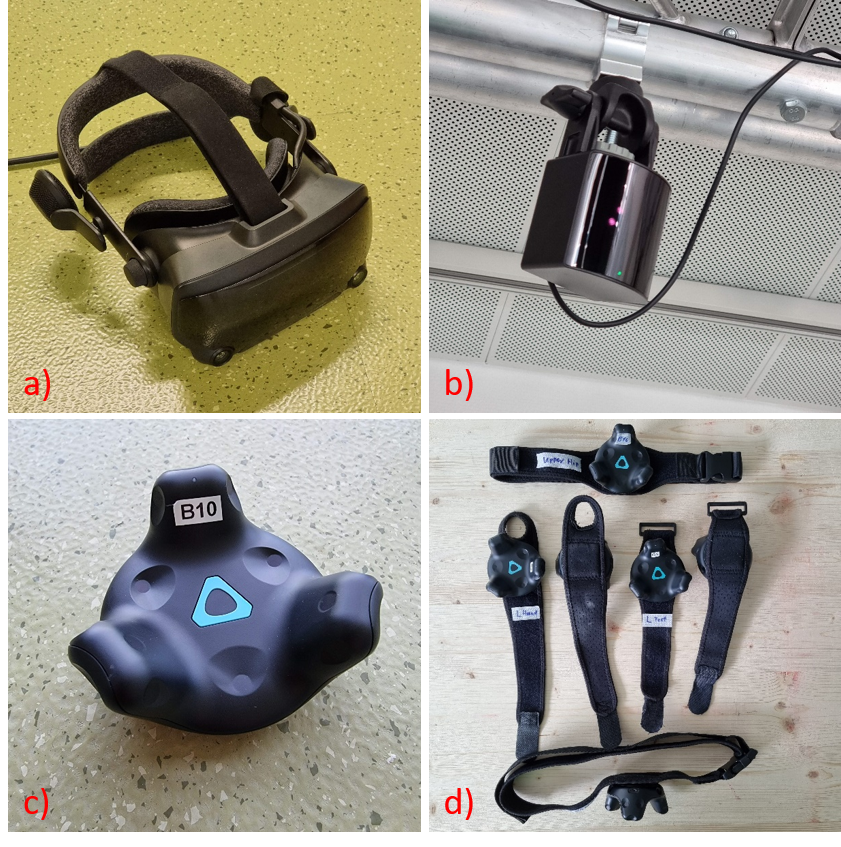
\includegraphics[width=0.8\textwidth]{figures/hardware.png}
	\caption[Hardware]{Hardware utilised by \exgo. a) Valve Index, b) base station, c) Vive Tracker 2, d) Vive Tracker 2 attached to Vive Tracker straps.}
	\label{fig:hardware}
\end{figure}

There are various options of devices to dive into Virtual Reality. Several devices have been evaluated, and the decision was made for the Valve Index\footnote{\href{https://www.valvesoftware.com/en/index}{https://www.valvesoftware.com/en/index}, accessed 29.3.2021} (figure~\ref{fig:hardware} a), because of its refresh rate, screen solution, field of view and the possibility to wear glasses underneath the head-mounted display (HMD). To determine the position and orientation of the HMD, the so-called Lighthouse is utilised. A Lighthouse consists of at least two base stations\footnote{\href{https://www.valvesoftware.com/en/index/base-stations}{https://www.valvesoftware.com/en/index/base-stations}, accessed 29.3.2021} (figure~\ref{fig:hardware} b). The base stations are placed at opposite corners of a room and span the tracking volume. To improve the tracking and for the avoidance of untracked areas, e.g. under the table, \exgo\ uses four base stations, one for each corner of the room, to span the Lighthouse.\\
With this setup, the learner can move in an empty virtual world. The next step is to replace the empty virtual world with a meaningful environment. To create the environment, the game engine Unity 3D\footnote{\href{https://unity.com/}{https://unity.com/}, accessed 29.3.2021} was used. In Unity3D, a basic room was created. Four light yellow walls, a parquet floor and unidirectional lighting. The parquet floor serves a purpose: it has a structure with frequent straight lines, making it easier to align the artefacts the learner will interact with. The room is kept simple not to distract the participant from the experiment.\\
Because high realistic GVs tend to perform better than abstract GVs~\cite{weber} and indicator-based GVs for full-body movements tend to overwhelm learners~\cite{lightguide}, the decision was made to used high realistic human-shaped avatars for the learner and the GV. The next step is to add the learner's avatar to the empty room. To achieve this, the learner's body needs to be tracked. Multiple full-body tracking systems were compared. The decision was made for Vive Tracker 2\footnote{\href{https://www.vive.com/eu/accessory/vive-tracker/}{https://www.vive.com/eu/accessory/vive-tracker/}, accessed 29.3.2021} (figure~\ref{fig:hardware} c), because of the cease of coordinate system matching, low latency and less work-intensive calibration process. The learner wears six Vive Trackers in total, compare figure~\ref{fig:tracker_placement}. Five of them plus the HMD are necessary for the full-body tracking of the learner. The remainder is necessary for RM (6.1), which is later explained in section~\ref{sec:logging}. Two trackers are located at Dorsum pedis\footnote{\label{fn:latin}Latin description: Dr. med. univ. Kilian Roth} (compare figure~\ref{fig:tracker_placement} a), two trackers are located at Dorsum manus\footref{fn:latin} (compare figure~\ref{fig:tracker_placement} b). One  tracker is located at Vertebra lumablis 5\footref{fn:latin} (L5) (compare figure~\ref{fig:tracker_placement} c). The trackers are attached to the learner by special Vive Tracker Straps\footnote{\href{https://www.google.com/search?q=vive+tracker+straps}{https://www.google.com/search?q=vive+tracker+straps}, accessed 10.03.2021} (figure~\ref{fig:hardware} d).\\
The Lighthouse tracks the Vive Trackers and HMD, which send their position to the PC. On the PC, SteamVR\footnote{\href{https://store.steampowered.com/app/250820/SteamVR/}{https://store.steampowered.com/app/250820/SteamVR/}, accessed 21.03.2021} receives the information and forwards it to Unity3D. In Unity3D, the SteamVR Plugin\footnote{\href{https://assetstore.unity.com/packages/tools/integration/steamvr-plugin-32647}{https://assetstore.unity.com/packages/tools/integration/steamvr-plugin-32647}} provides the information in a workable format. The tracking information is now about to be transformed into a rendering of a human-like avatar at the position of the learner's body. This requires several steps.\\First, an avatar is imported. To create the avatar, Reallusion Character Creator 3\footnote{\href{https://www.reallusion.com/character-creator/}{https://www.reallusion.com/character-creator/}, accessed 21.3.2021} was used. To match the gender of the participant, a male and a female character was created, wearing the same clothes. Based on the demographic questionnaire, the gender can be set, and the participant will see an avatar complying with the participant's gender.\\
Secondly, the tracker's position and orientation in the tracking volume have to be translated into humanoid movements that meet the learner's movements. This is achieved by Inverse Kinematics (IK).\\
\begin{figure}[htb]
	\centering
	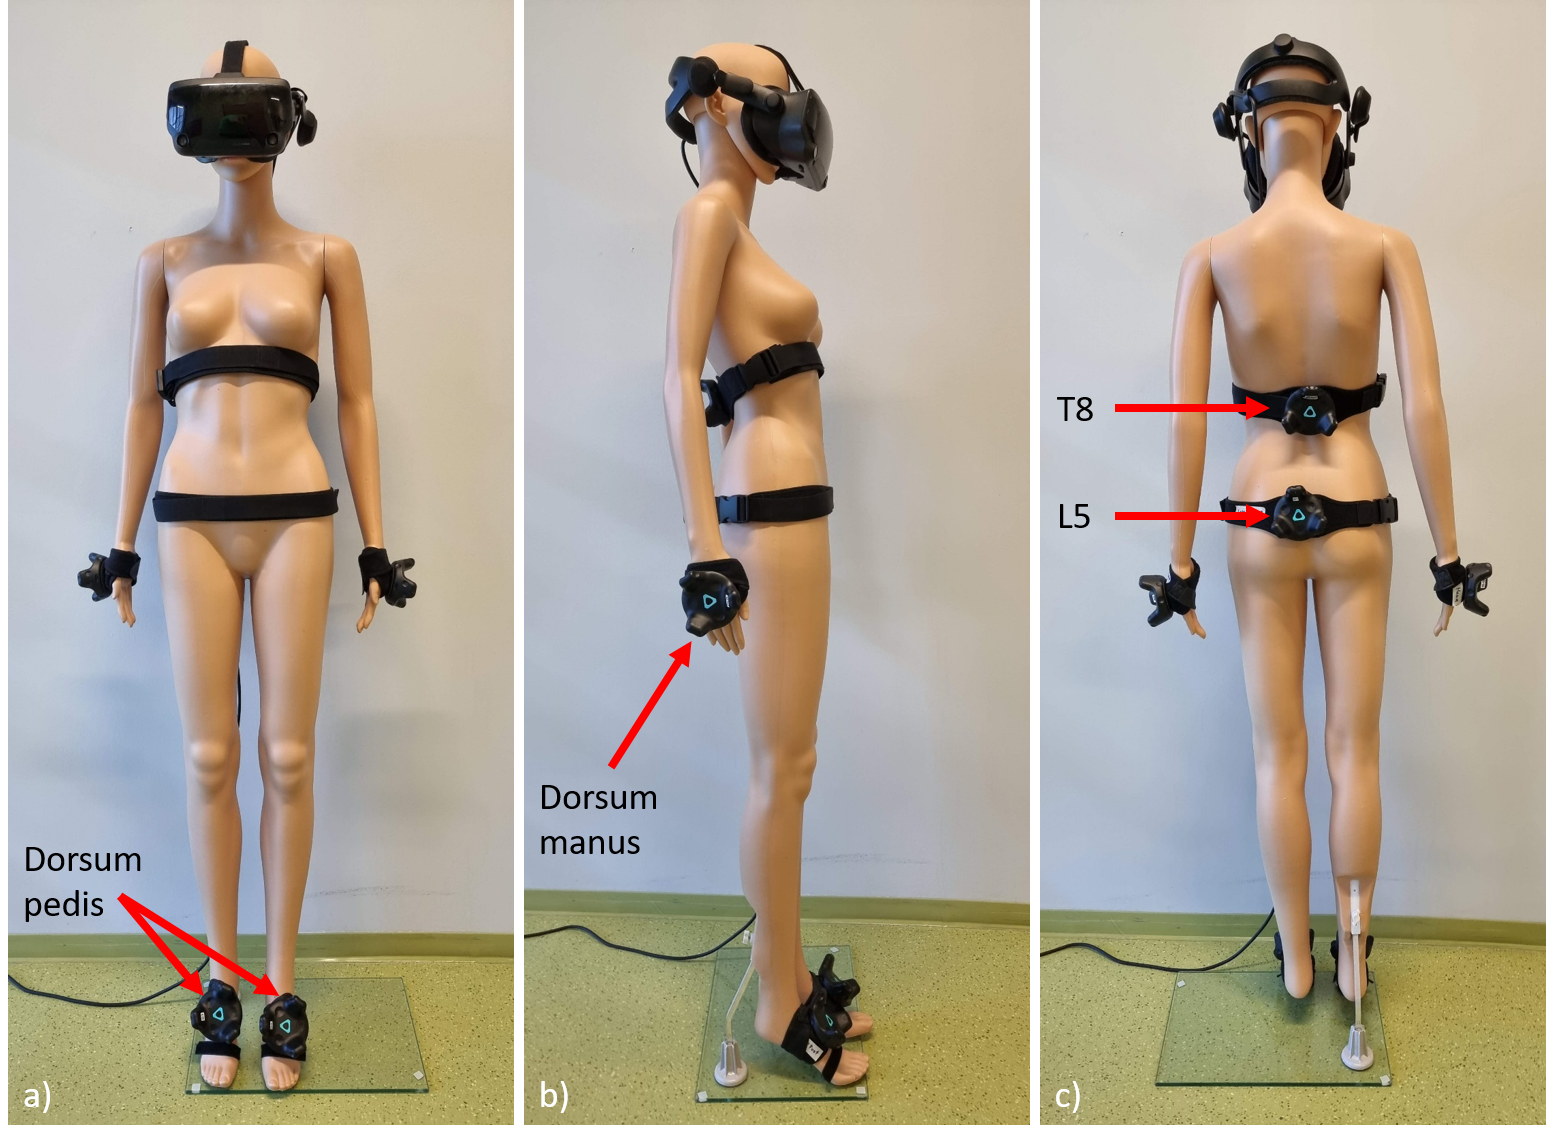
\includegraphics[width=\textwidth]{figures/trackerPlacement.png}	
	\caption[Tracker placement]{Tracker placement. a) front view - Vive Tracker at Dorsum pedis, b) side view - Vive Tracker at Dorsum manus, c) back view - Vive Tracker at Vertebra lumablis 5 (L5) and Vertebra thoracalis (T8).}
	\label{fig:tracker_placement}
\end{figure}
Short excursion: IK arises from the field of robotics. A robot arm consists of limbs and joints. Each limb has a specific length, and each joint has a specific range of angles to move. The length and angles are called rules. Given an endpoint the robot has to reach with the most outer limb, the angle of each joint can be calculated with the rules. This process can be mapped to a human body, too.\\

Unity3D provides a third-person plugin called FinalIK\footnote{\href{https://assetstore.unity.com/packages/tools/animation/final-ik-14290}{https://assetstore.unity.com/packages/tools/animation/final-ik-14290}, accessed 21.03.2021} that is capable of the calculations in question. On the one hand, FinalIK is powerful and unrivalled in functionality compared to other IK tools and thus influenced the choice to use Unity3D for \exgo\. On the other hand, to match the needs of the experiment, extensive adjustments were necessary. The main task is to transfer the information from SteamVR to FinalIK in a meaningful way so that FinalIK animates the learner's body faithfully.\\
SteamVR registers the Vive Tracker in the order they are switched on. To increase the reliability of \exgo, a script was created that assigns the tracker by the hardware ID. The trackers are then assigned to a script called VRIKCalibrationController. The VRIKCalibrationController matches the tracker with the avatar and resizes the avatar to the learner's height. FinalIK is constructed to work with controllers in the user's hands. In \exgo, the experiment participants needs the hands to interact with the box, thus the controllers are replaced with Vive Tracker on the back of the hands. Shifting the reference points of the hands yields a faithful representation of the learner's hands. The feet needed similar adjustments. Finally, FinalIK is able to solve the movements. Solving is the process of translating the tracker information into an animated avatar. For clarification, the complete rendering pipeline exemplary for the hip of the learner is attached in appendix~\ref{a:studentRenderingPipeline}.\\
FinalIK requires calibration before use. For calibration, the person equipped with the trackers needs to perform a T-pose facing a specific direction. To ease the calibration process, a virtual mirror is placed in the room. The participant can be asked to look into the mirror and expand the arms, leading to the participant's correct orientation during the calibration process. Immediate with the calibration, the mirror disappears.\\
After the calibration, the system is ready to start with the task. Because the participant is now standing in front of the mirror, the position in front of the mirror is chosen as the starting point and endpoint of every task.\\
With the steps implemented in this section, the outcome results in a faithful representation of the learner, see figure~\ref{fig:selfPerception}.\\

The approach of translating a real-world person to the digital world with the help of Vive Trackers and IK was used by other researchers, too, for example~\cite{samesetup,perspectivematters}. 

\begin{figure}[H]
	\centering
	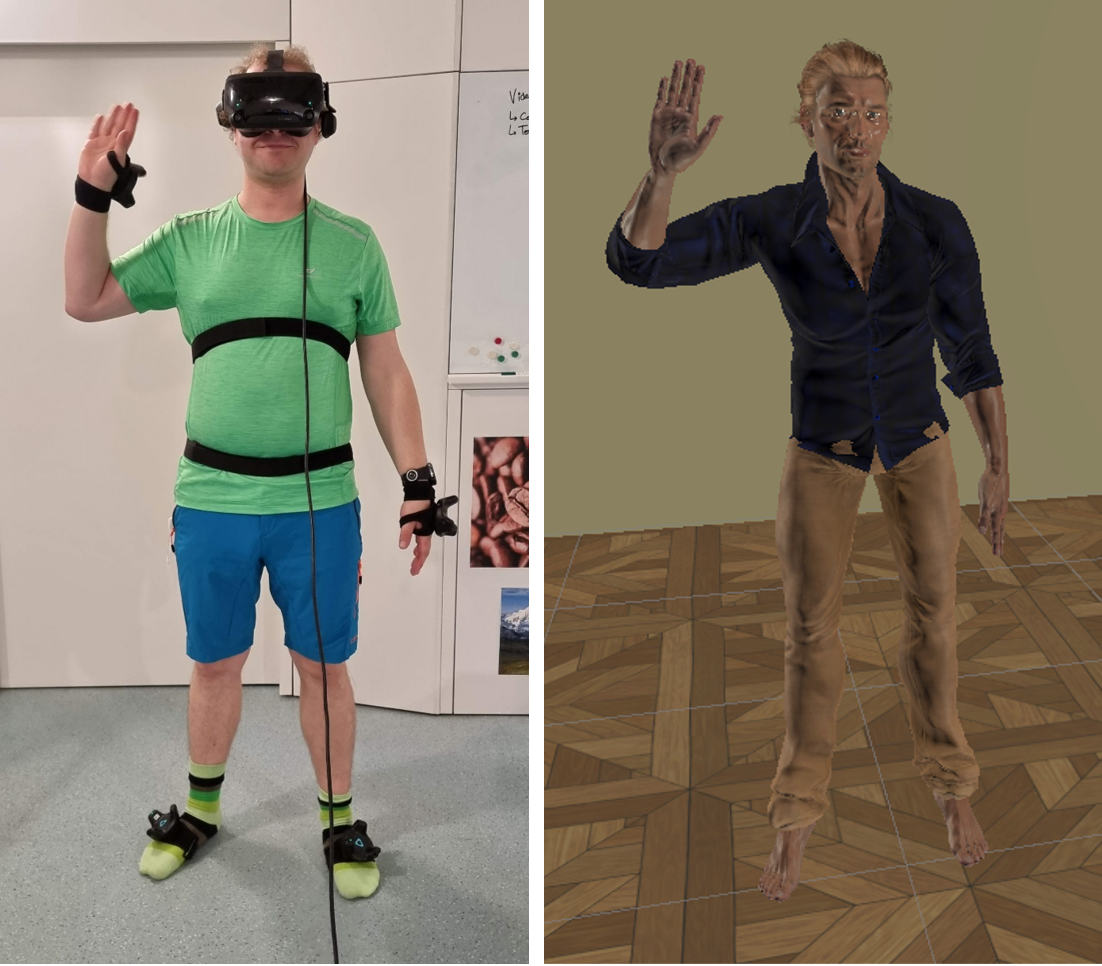
\includegraphics[width=\textwidth]{figures/selfPerception.png}	
	\caption[Digital representation of real-world person.]{Digital representation of real-world person with \exgo. a) real-world person, b) digital avatar representation in VR of the real-world person. Images not taken at the exact same time.}
	\label{fig:selfPerception}
\end{figure}

\section{Physical Artefacts}
\label{sec:artefacts}
\begin{figure}[H]
	\centering
	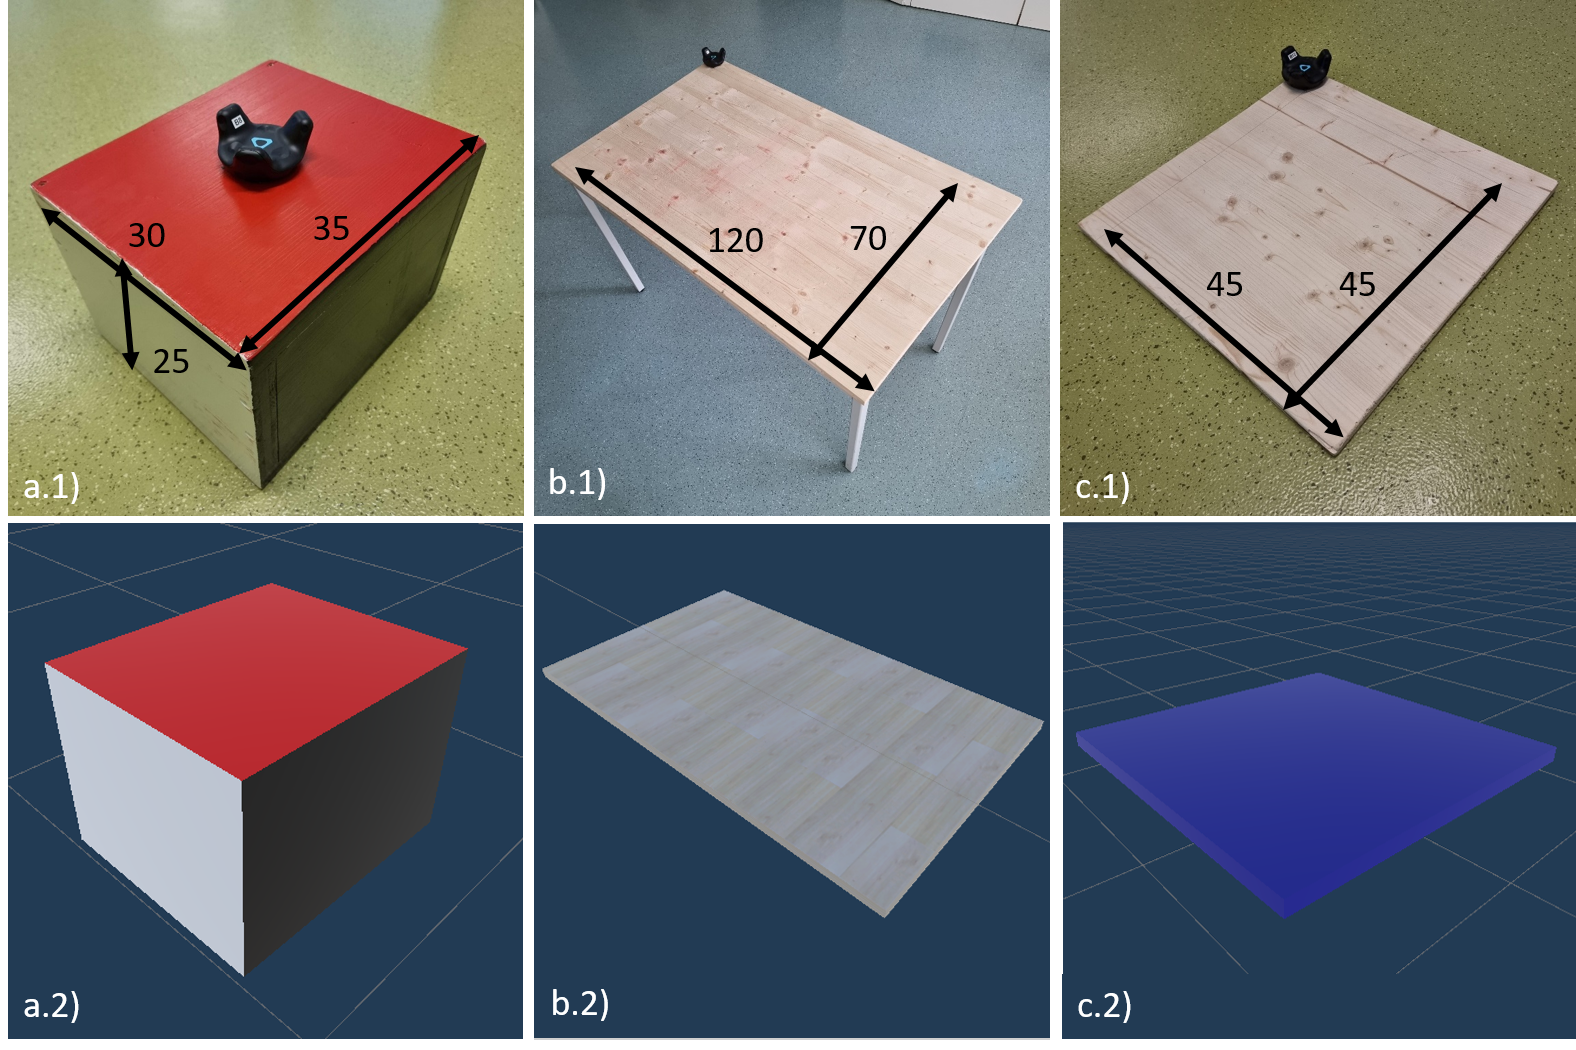
\includegraphics[width=\textwidth]{figures/artefacts.png}	
	\caption[Artefacts of \exgo]{Physical and corresponding digital artefacts of \exgo\ including measures in cm. a) box, b), table --- measures do not include the additional 6cm to attach the tracker, c) scale --- measures do not include the additional 5cm to attach the tracker.}
	\label{fig:artefacts}
\end{figure}
With the previously described elements in place, the learner can see the own body in an empty room. The task includes the handling of physical load on a table and a scale. The creation of the table, scale and the box, which will serve as physical load, starts with the construction of them - physically and digitally. Figure~\ref{fig:artefacts} shows the physical and digital versions of the box (a), table (b) and scale (c).\\
The first version of \exgo\ used a cardboard box (27cm x 26cm x 24cm) as physical load. During the development, it became clear that the size of thecardboard box was too small and light to serve as a physical load. To determine a suitable size, several boxes of different dimensions were informally tested. With nine different boxes, a set of subtasks were performed. The major insight from this test was that the length of the box' sides should be unequal to see the direction of the box visually. Furthermore, the box should be perceived as physical load by having a reasonable size and a certain weight. Simultaneously, the box should not be too heavy and thereby limit the experiment participants to strong humans or being a threat to the participants' bodies. The sizes were set for 35cm x 30cm x 25cm. The measures of the box differ by 5cm in every dimension. This makes it clear to see the orientation of the box. The final box was constructed from three-layered wood with a strength of 27mm. The resulting weight was 5.8kg. To evaluate the weight of the box, one male participant\footnote{Evaluation with at least one male and one female person is desirable. This was not possible because of the COVID-19 pandemic.} was asked to perform all subtasks. The participant is a computer science PhD student and experienced with several sports activities. Observations revealed no incidences that contradict to use the box as physical load: the box could be safely held in hands, and it was visible that the person changed the own posture during the handling of the box to perform the movements more ergonomically. The posture change can be interpreted as a sign that the box is perceived as "load". The person rated the weight as "ok". He had no problems moving the box.\\
The box was painted in three high contrast colours: black, white and red. Each opposite side was painted in the same colour. The painting facilitates the visual perception of the orientation of the box. The digital pendant of the box is a cuboid in the same colour and size. To translate the physical box' position and orientation to the virtual one, a Vive Tracker is attached to the box and fixated with a screw. The plus side of using a screw is the prevention of any relocation of the tracker. The downside is that tremors caused by placing the box on, for example, the table, are transferred directly into the tracker. This causes the tracker to lose tracking. To interrupt the transfer of tremors, shock-absorbing insulation is placed between the tracker and the box.\\
During the development of \exgo\, an office table (120cm x 60cm x 72cm) was used. The digital pendant to the physical table is a plate in the same size and colour as the tabletop. The position and orientation of the table are assessed by a Vive Tracker. Unfortunately, the tracker was placed on the top of the table inside the working area, where the box will be placed and shifted during the tasks. To shift the tracker out of the working area, a new tabletop was constructed. Because the used office table was too narrow, the width was increased by 10 cm. The new tabletop is out of three-layered wood, with an additional increased size of 6cm in length and width (126cm x 76cm instead of 120cm x 60cm) to provide additional space for the tracker. The tracker is attached on the most outer edge, thus out of the working area. To prevent tremors from passing from the table into the tracker, shock-absorbing insulation is applied between the tracker and tabletop.\\
The last artefact to create is the scale. The scale is a waypoint in the room where the participants perform \textit{lift} and \textit{lower} to the ground. The scale is a rectangular plate of 45cm x 45cm so that the box can be placed on the scale easily. To shift the tracker out of the area where the box will be placed, the plate is extended by 5cm. The tracker is attached to the most outer edge of the extension with a screw and shock-absorbing insulation. The digital pendant is a plate with the exact dimensions of the physical plate, excluding the extended area. The physical artefacts were constructed and built by myself.\\

\section{Experiment Setting}
\label{sec:experimentSetting}
\begin{figure}[H]
	\centering
	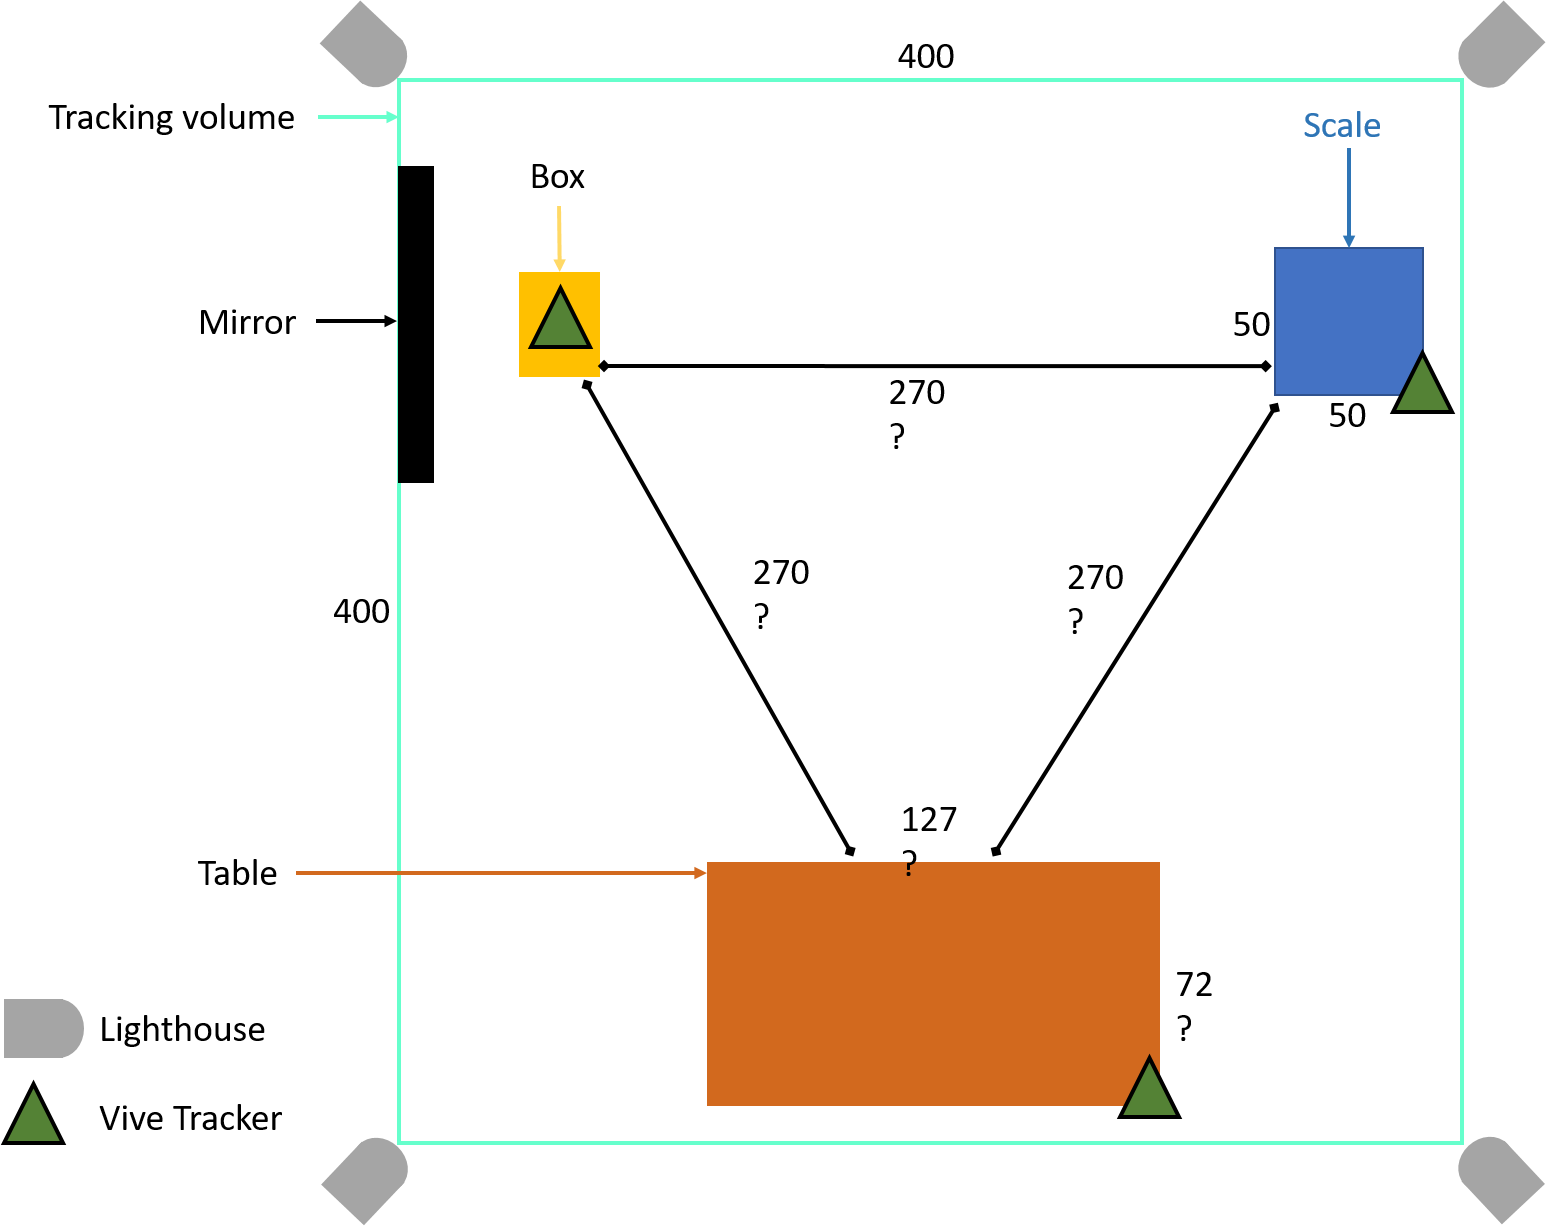
\includegraphics[width=\textwidth]{figures/study_setting.png}
	\caption[Experiment setting]{Experiment setting with measures in cm.}.
	\label{fig:study_setting}
\end{figure}
Meanwhile, \exgo\ consists of a room, an avatar representing the learner, table, box and scale. In the following, an overview of the alignment of these elements is given. Figure~\ref{fig:study_setting} shows the sylised virtual room in which these elements are aligned. Figure~\ref{fig:learner_positions} show the corresponsing real-world room. All positions that are described in the task description (compare table~\ref{tab:tasks}) are depicted. The outer line represents the Lighthouse or tracking volume, which is approximately 400cmx400cm.\\
On the left wall, the mirror is located. In front of the mirror, the starting and end position of the box is seated. Beside the box is the position \textit{mirror}, the start and endpoint of each task. The table is placed in the middle of the wall to the left of the mirror. Around the table, the positions \textit{table centre}, \textit{table right} and \textit{table left} are located. At the opposite wall of the mirror, the scale is placed. In front of the scale is the position \textit{scale}.
\begin{figure}[htb]
	\centering
	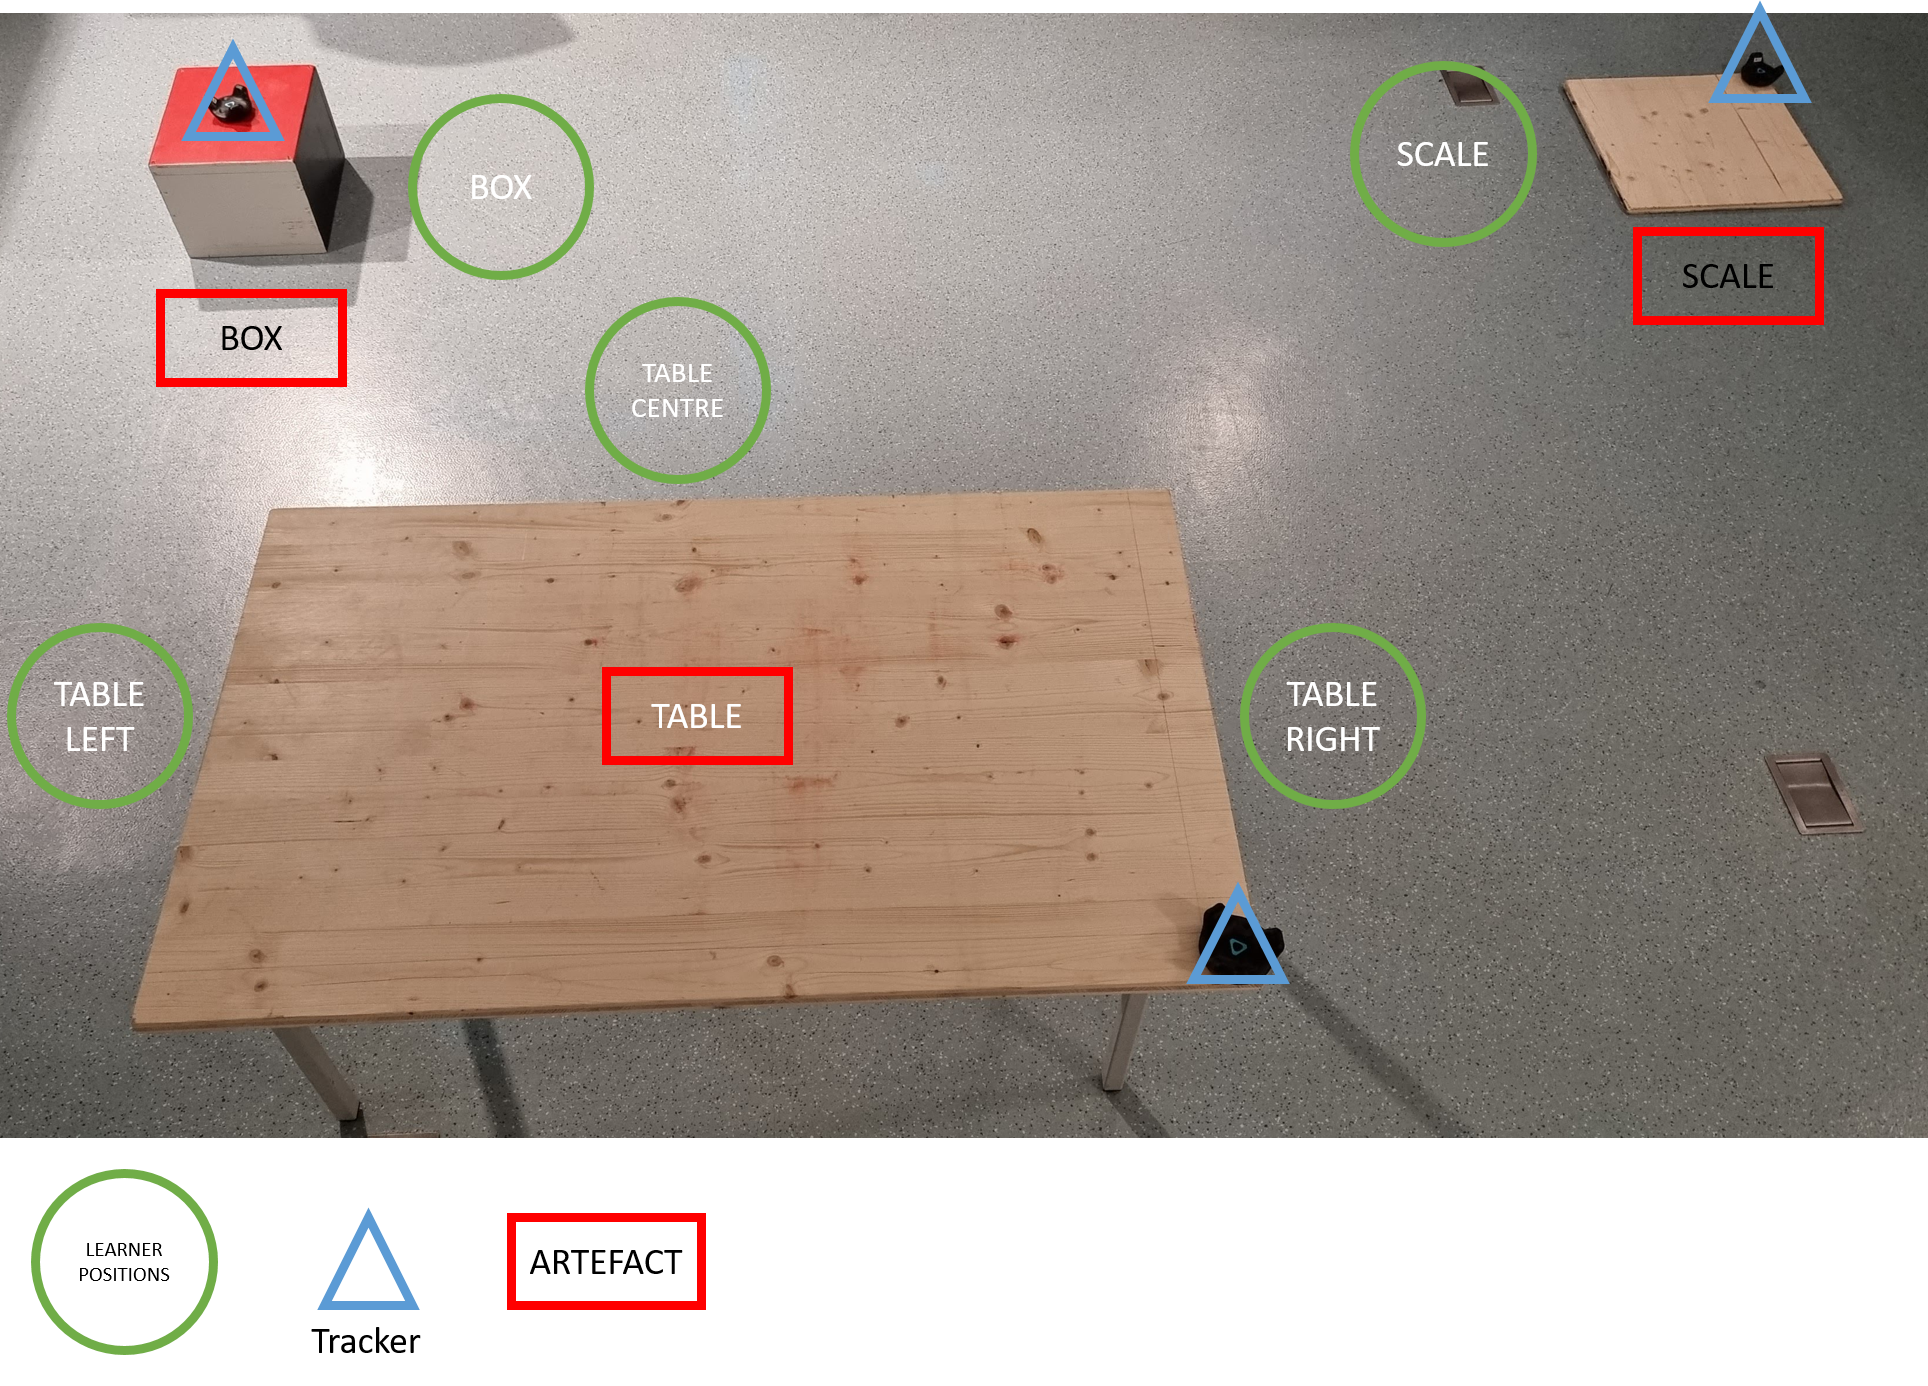
\includegraphics[width=\textwidth]{figures/learner_positions.png}
	\caption[Learner positions]{Learner positions. Green circles indicate positions of the learner mentioned in the task description in table~\ref{tab:tasks}. Red suqares mark artefacts, blue triangles mark Vive Trackers}
	\label{fig:learner_positions}
\end{figure}

\section{Guidance Visualisation}
\label{sec:gv}
The next task is to add the GV to \exgo, which the learner will mimic. The GV is an avatar like the learner's avatar, with the difference that the motion of the GV is driven by the pre-recorded tasks 1-3. The recording of the tasks was also performed with \exgo. To use \exgo\ as a recorder, a copy of all trackers and the HMD is created. This recorder-copy is packed in one GameObject with the trackers as children. The parent GameObject is recorded during the performance of the movements. For the GV, a similar GameObject as the recorded GameObject is created and serves as Input for FinalIK. In this section, the main points of the process are described: the recording of the movements and the resizing of the GV to the size of the learner.\\

The movements in the task have to be performed ergonomically. The measures to evaluate ergonomic movements are the RM. To serve as a strong baseline, a professional for ergonomic movements should record the movements. Because of the COVID-19 pandemic, all attempts to record the movements by a professional failed. The whole laboratory was transported to a private facility, but because of temporal issues, the recording with the professional could not take place. Then the laboratory was transported to another private facility. Unfortunately, the room in which the laboratory was set up was not suitable for the recordings. The recorded movements by the professional had to be abandoned because of insufficient tracking coverage causing jitter. The laboratory was transported back to the university. Eventually, I was trained by a physiologist and recorded the movements by myself. The final recordings were examined by the physiologist. Overall, the movements were rated by the physiologist as "by and large correct". The back is not always straight or at the correct angle. In task 2 during a \textit{push} and in task 3 during a \textit{pull}, the feet are misplaced.\\

With the recording of the tasks at hand, the GV can be animated. For the ego-centric VP it is inevitable that GV and learner have the exact same size. Otherwise, the learner cannot perceive the GV correctly. Furthermore, the table, box, and scale must not resize. The solution is to record two sets of object synchronously. The first set contains the objects that have to be resized, namely the GV, the second set contains objects that must not be resized, namely the box, table and scale. The recordings were synchronised by a script, the playback of the animations in \exgo, too. The resizing of the GV takes place in three steps, compare figure~\ref{fig:resize}. First, the learner and the GV are calibrated. Then the height difference $\Delta y$ is measured between the learner and GV. In the last step, FinalIK is removed from the GV, the animated GameObject containing all trackers is removed, then FinalIK reattached and calibrated with the resized GameObject containing all trackers. After this process, learner and the GV have the same size.
\begin{figure}[htb]
	\centering
	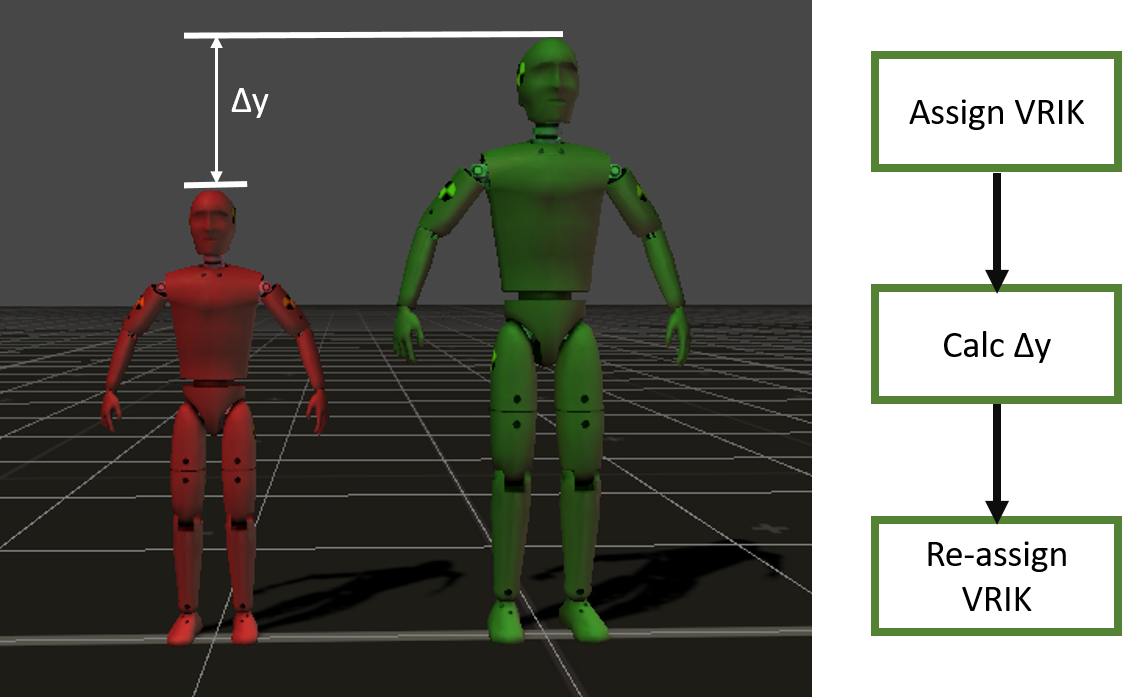
\includegraphics[width=\textwidth]{figures/resize.png}
	\caption[Resizing the GV to the learner's height.]{Schematic description of the process to resizing the GV to the learner's height.}
	\label{fig:resize}
\end{figure}

\section{Visual Perspectives}
\label{sec:perspectives}
The next element to add to \exgo\ are the VPs the experiment will compare, namely the ego-centric VP, the exo-centric VP and the ego- \& exo-centric VP. The implementation of the VP is partly informed by Chua et al.~\cite{thaichichua}. Chua et al. used full-body high realism degree avatar representations as GVs teaching stationary Tai Chi. In the ego-centric VP, the GV is placed inside the learner's avatar. In the exo-centric VP Chua et al. decided to placed the virtual copy of the learner and the GV side by side.\\

The ego-centric VP requires, besides the learner, one ego-centric GV. The learner needs to stay inside the GV. This is achieved by the \textit{speed mechanic}, compare section~\ref{sec:mechanics}. The learner's distance to the GV is calculated with the help of the tracker at the hip of the learner and the recorded tracker at the hip of the GV. The positions of the trackers at the hip are projected to the floor. The projection to the floor is necessary because the \textit{speed mechanic} would apply if the GV bends the knees during \textit{lift} and \textit{lower}: if the GV bends the knees and the learner does not, the distance will increase between the two trackers in the y-component. This restricts the learner's ability to perform an error: if the learner does not bend the knees during \textit{lift} and \textit{lower}, the GV would stop and remind the learner to bend the knees. To investigate if the learner could percept to bend the knees, the learner must be allowed to make this error. This is why the \textit{speed mechanic} relies on the distance between the two projected points on the floor.\\
Additionally, the distance used for the \textit{speed mechanic} finds application in another functionality. In the ego-centric VP, the learner is located inside the teacher. This means that the learner's viewport is inside the head of the GV and let the learner see the inside of the GV head. This leads to distraction due to the partly rendered inner head. The solution is to remove the head rendering if the distance is below $ETD_{max}$ and reinitiate the rendering above $ETD_{max}$. The rendering is removed by replacing the materials array of the head with a material array that contains only invisible materials. Figure~\ref{fig:ego} visualises the ego-centric VP by showing the bird's-eye view (top) and the view from the first-person perspective (bottom).\\

In the exo-centric VP, four exo-centric GVs are located around the learner. The positions of the exo-centric GV were determined after the task was recorded. The difficulty is to determine proper positions of the exo-centric GVs. First, at any point in time during every task's performance, the learner must be able to see a GV by only turning the head. Secondly, the GV and the learner should not move through a table or scale of another GV. The solution to the first part is informed by Chua et al.~\cite{thaichichua}. Chua et al. chose four representations that are in front, behind, left and right of the central learner. The second part proved to be impossible if the exo-centric representations should be near enough to be observed by the learner. A GV crossing through an artefact of another GV happens rarely and only during the subtask \textit{carry}, but is a limitation of \exgo. The GV needs to be shifted too far away from the learner not to cross other GVs artefacts. In a distance in which no crossing occurs, the movements are barely visible to be mimicked correctly. The exo-centric representations were then placed at a distance that allows being observed by the learner, and the learner can access all positions without standing in a digital artefact of another GV. The exo-centric GVs are positioned as follows. Standing at table centre and looking in the direction of the table: the GV to the left is shifted by two meters to the left, the GV to the right, two meters to the right. The GV in front is shifted by 1.5 meters to the front. The GV in the back is shifted 3 meters to the back. Figure~\ref{fig:multireppositions} shows the positions of the exo-centric VP. Additionally, to the exo-centric GVs, a virtual copy of the student needs to be rendered. The same values shift the virtual copy of the learner. Figure~\ref{fig:exo} visualises the exo-centric VP by showing the bird's-eye view (top) and the view from the first-person perspective (bottom).\\

In the last VP, the ego- \& exo-centric VP, the learner has an ego-centric VP and the exo-centric GV with the corresponding virtual copies of the learner. The implementation of the ego- \& exo-centric VP is the union of the implementations of the ego-centric VP and exo-centric VP. Figure~\ref{fig:egoexo} visualises the ego- \& exo-centric VP by showing the bird's-eye view (top) and the view from the first-person perspective (bottom).\\
\begin{figure}[htb]
	\centering
	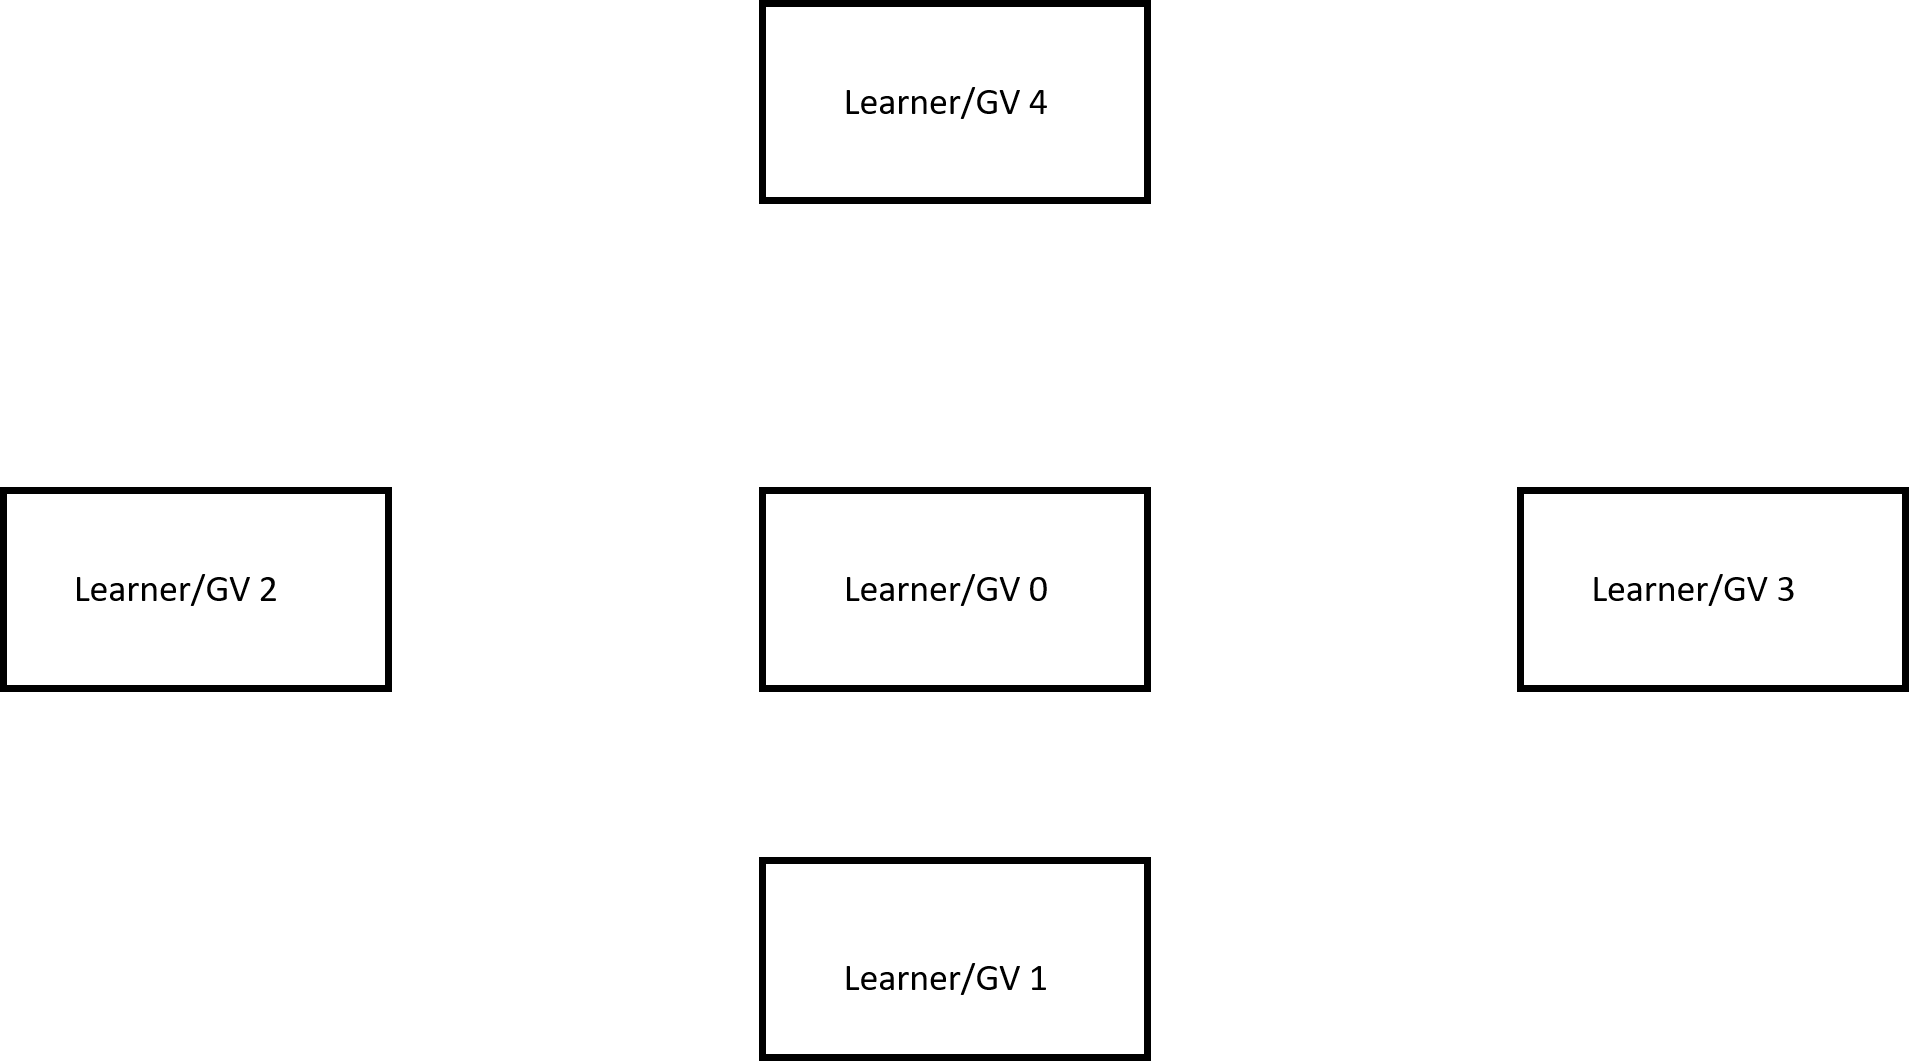
\includegraphics[width=\textwidth]{figures/positions.png}
	\caption[Positions of representations.]{Position of representations.}
	\label{fig:multireppositions}
\end{figure}
\begin{figure}[H]
	\centering
	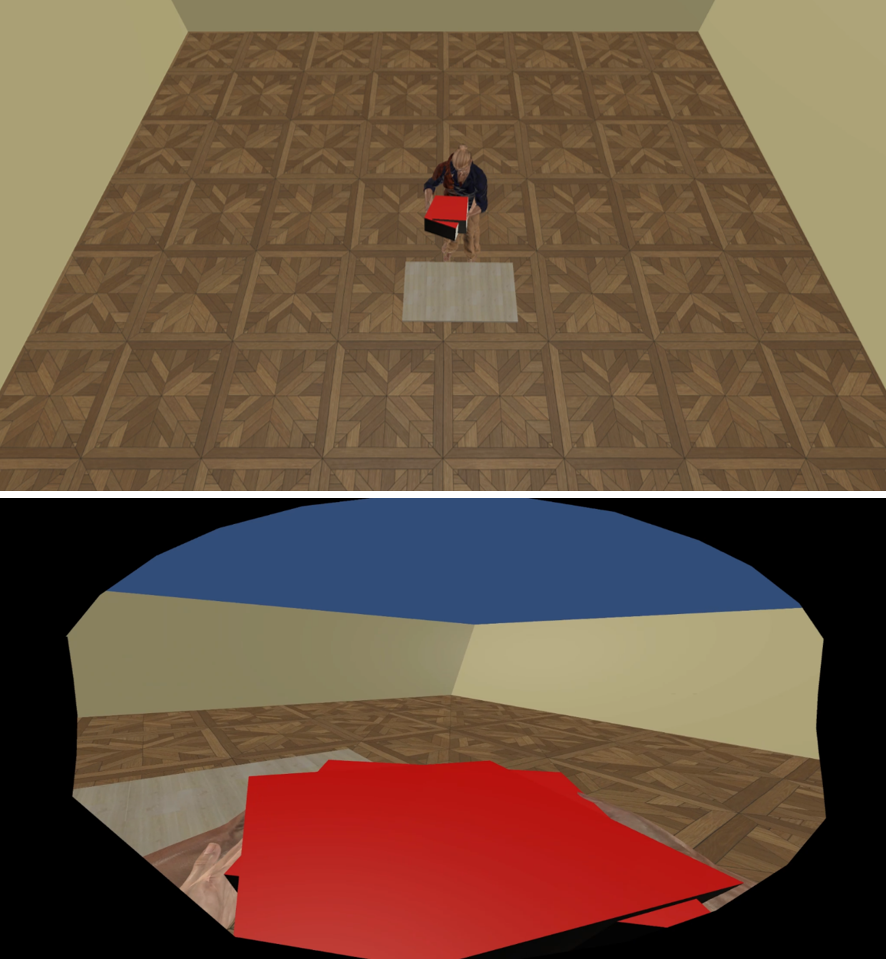
\includegraphics[width=\textwidth]{figures/perspectiveEGO.png}
	\caption[Ego-centric visual perspective]{Ego-centric VP from the bird's-eye view (top) and ego perspective (bottom) on the exact same scene. The GV (woman in red shirt) in located inside the learner (man in blue shirt).}
	\label{fig:ego}
\end{figure}
\begin{figure}[H]
	\centering
	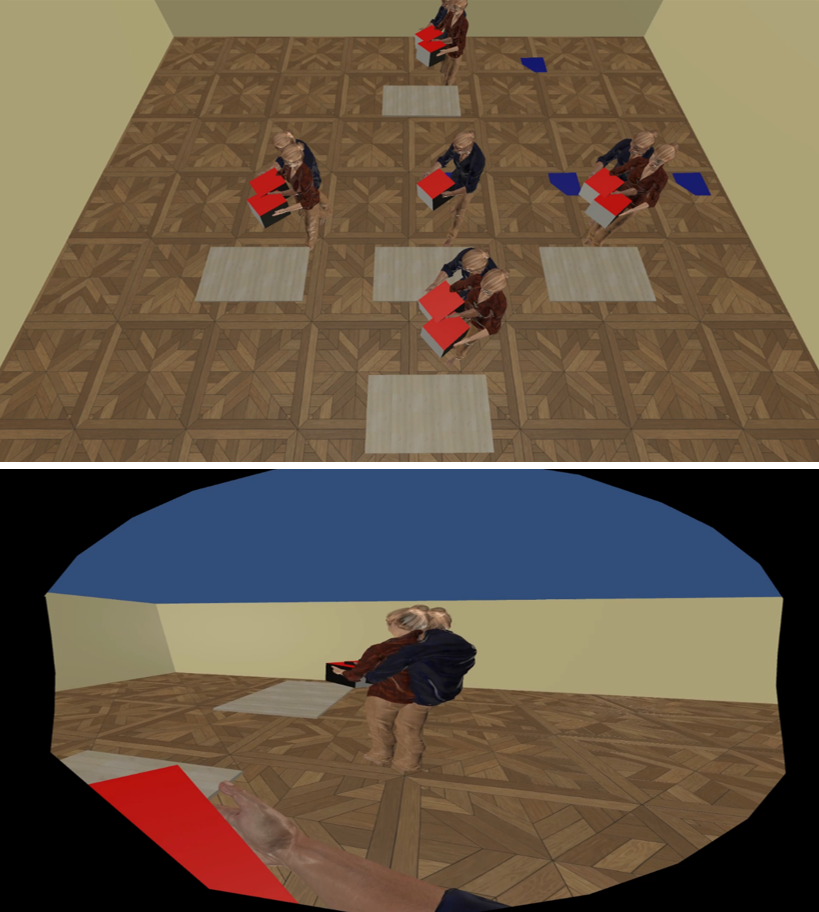
\includegraphics[width=\textwidth]{figures/perspectiveEXO.png}
	\caption[Exo-centric visual perspective]{Exo-centric VP from the bird's-eye view (top) and ego perspective (bottom) on the exact same scene. The GV's (woman in red shirt) are located around the learner (man in blue shirt). Additionally, a virtual copy of the learner is located inside the exo-centric GVs.}
	\label{fig:exo}
\end{figure}
\begin{figure}[H]
	\centering
	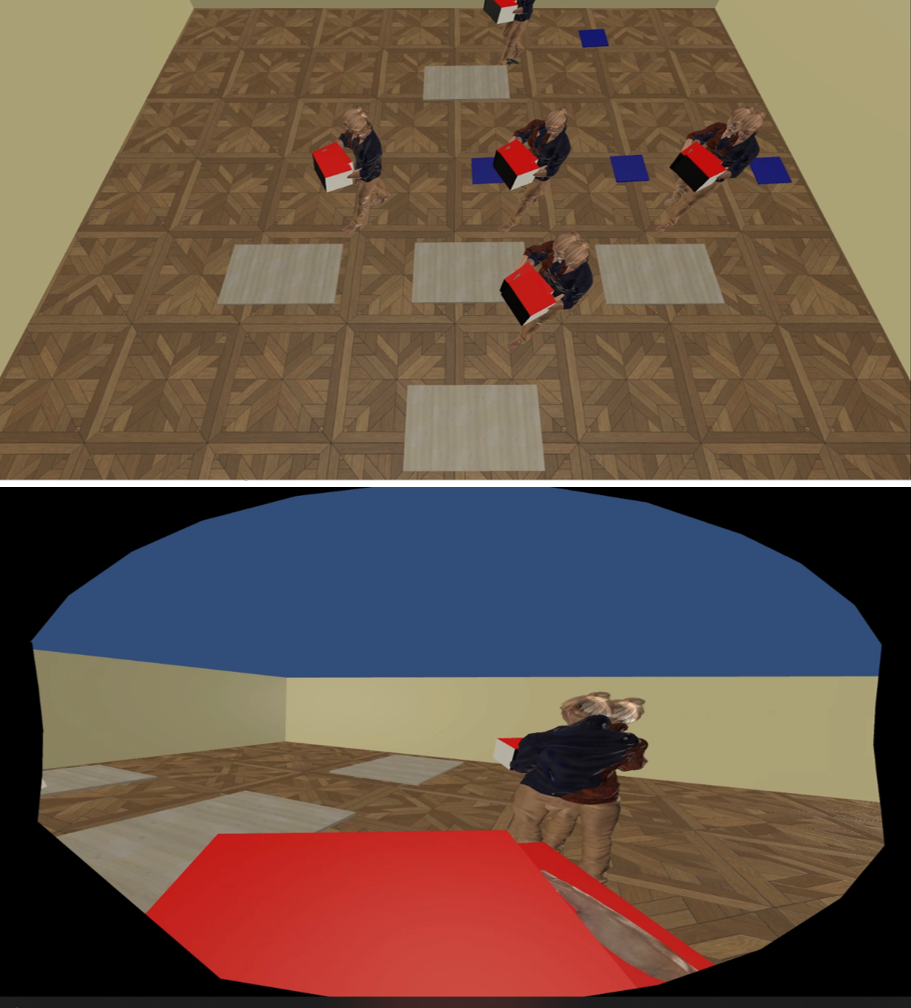
\includegraphics[width=\textwidth]{figures/perspectiveEGOEXO.png}
	\caption[Ego- \& exo-centric visual perspective]{Ego- \& exo-centric VP from the bird's-eye view (top) and ego perspective (bottom) on the exact same scene. The GV's (woman in red shirt) are located around the learner (man in blue shirt) as well as inside. Additionally, a virtual copy of the learner is located inside the exo-centric GVs.}
	\label{fig:egoexo}
\end{figure}

\section{Quantitative Data Aquisition}
\label{sec:logging}
\begin{table}[H]
	\centering
	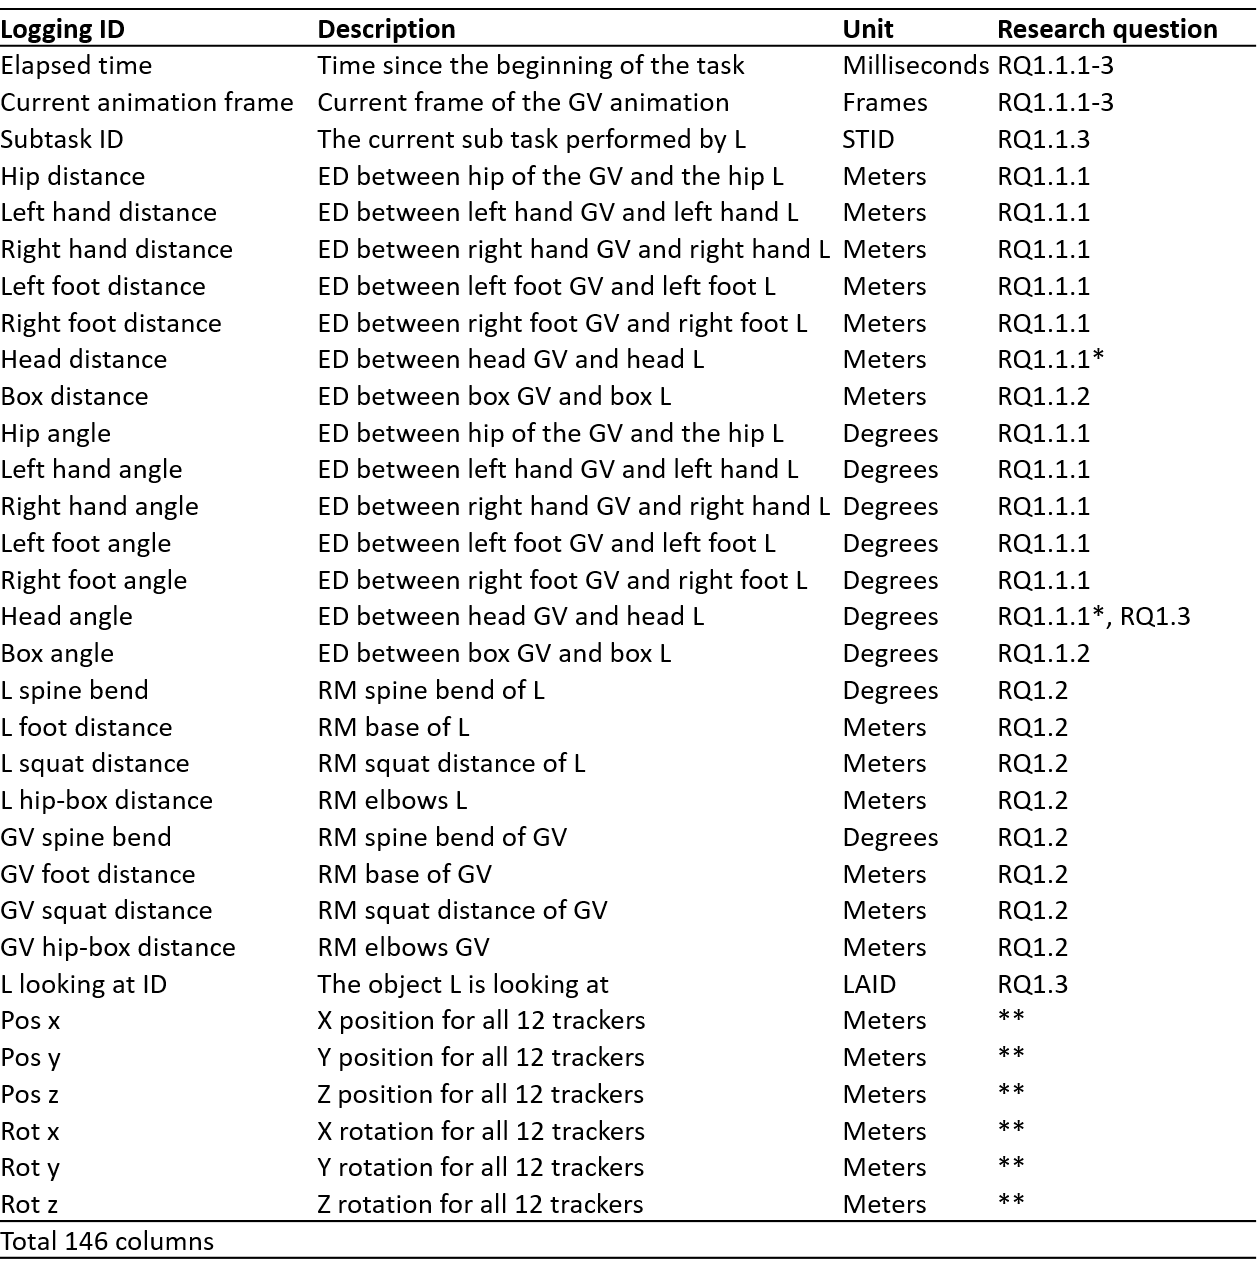
\includegraphics[width=\textwidth]{figures/logging_detail.png}
	\caption[Logfile description]{Detailed overview of logs produced by \exgo\ per frame. L: learner, GV guidance visualisation, ED: euclidean distance. *head position and rotation is biased in exo-centric conditions because of multiple GV the L can focus on. **All trackers are logged for backup reasons: after the experiment is conducted, a measurement can become interesting that was not of importance before. With these values, any measurement can be calculated post-experiment.}
	\label{tab:logging_detail}
\end{table}
Section~\ref{sec:measures} defined the measures that are necessary to answer the research questions. \exgo\ must be capable of assessing all measures. This section explains how \exgo\ assesses the measures. An overview of all measures is listed in table~\ref{tab:logging_detail}. Table~\ref{tab:logging_detail} lists the logging ID, a description of what the measurement is measuring, the unit in which the measurement is measured and for which research question the measurement is assessed. Quantitative data acquisition can be divided into several classes: (i) accuracy measurements (1-5), (ii) ergonomic measurements (6), (iii) focus measurement (7) and (iv) time measurements (9). In the following, (i)-(iv) are discussed.


\subsection{(i) Accuracy Measurements}
The accuracy measurements assess the discrepancy between the movements of the learner and the movements of the GV. Accuracy measurements are subdivided into distance-based measures and angle-based measures. Distance-based measures rely on the Euclidean distance between the learner's body parts and the body parts of the GV. The reference point for the body part is the tracker, which is attached to the body part. The body parts are: hip, left hand, right hand, left foot, right foot and head. The distance between the learner's box and the box of the teacher is an accuracy measurement, too. Similar to the body parts, the distance between the two boxes is the Euclidean distance between the tracker of the box and the recorded tracker of the GV. Please note, the trackers are not visible to the learner during the experiment.\\
Angle-based accuracy measurements assess the discrepancy in orientation between the body parts and box of the learner and the GV. The angles are measured in degrees. The calculation of the angle-based measurements complies with the calculations of the distance-based measurements. This means the angle between the corresponding trackers is measured. To summarise: distance-based measurements assess the positioning's error, angle-based measurements assess the error in orientation. Similar accuracy measurements are used by~\cite{onebody,thaichichua,YouMove,physioathome,vrdancetrainer,lightguide}.

\subsection{(ii) Ergonomic Measurements}
\label{sec:ergonomicMeasurements}
\begin{figure}[H]
	\centering
	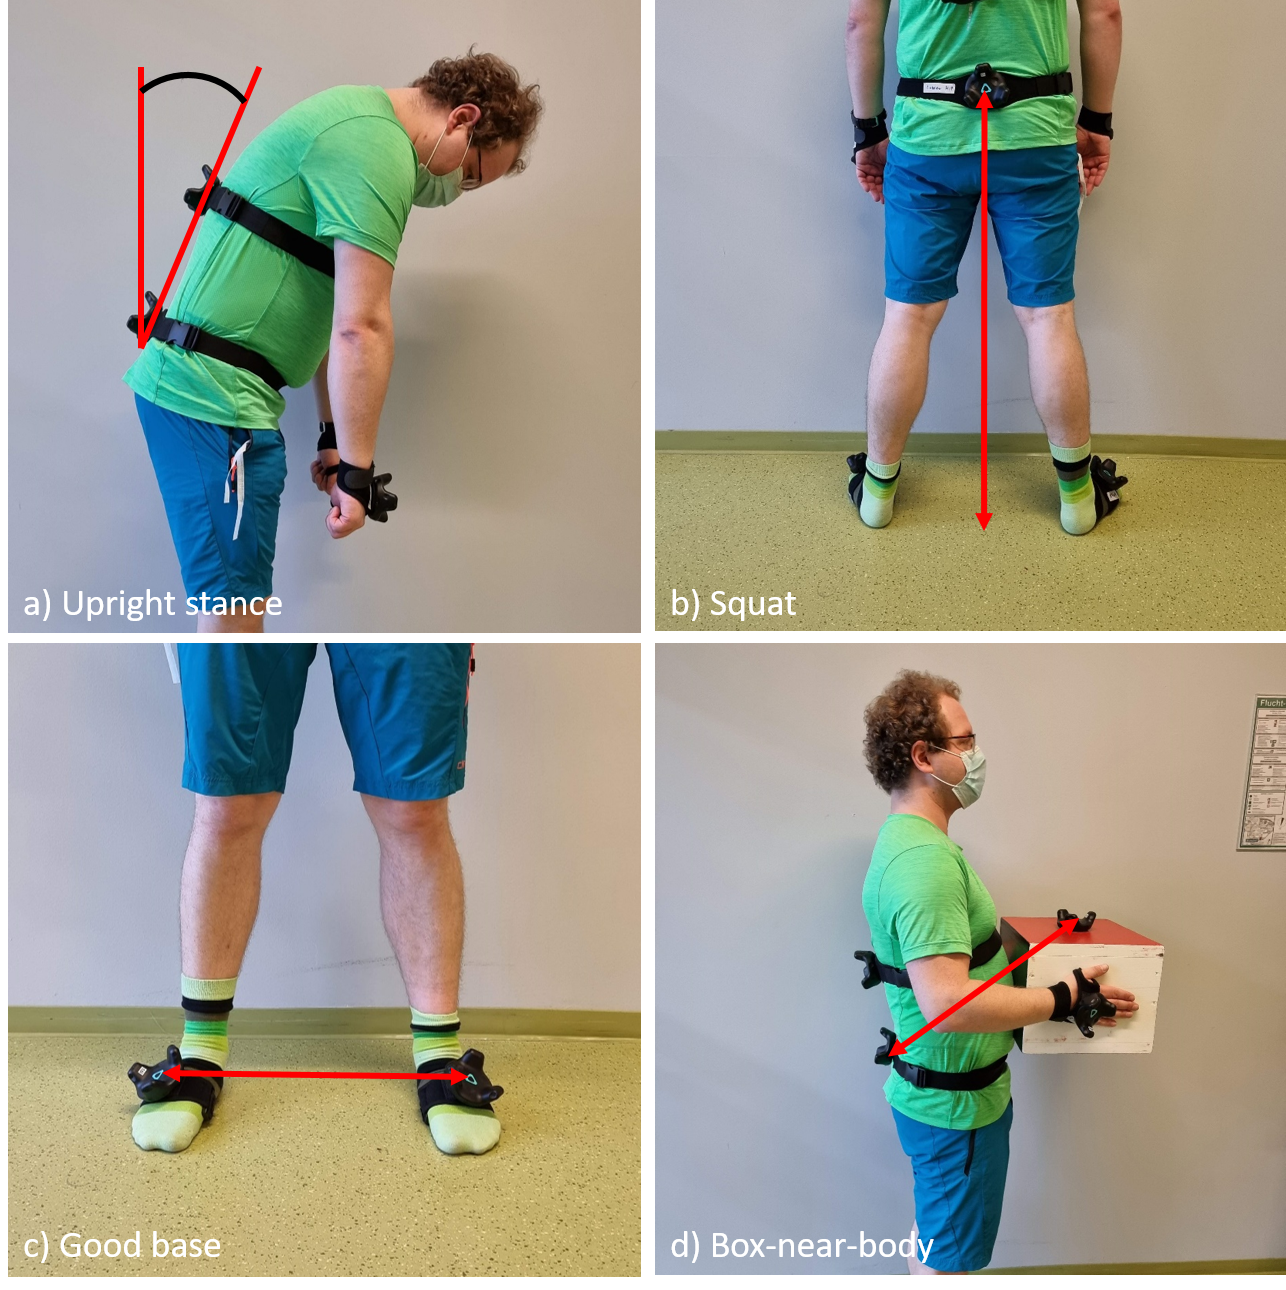
\includegraphics[width=\textwidth]{figures/riskMeasurements.png}
	\caption[Risk metrics calculation]{Calculation of the risk metrics. a) \textit{upright stance} --- angle between the upright vector and the vector from the L5 tracker to the T8 tracker, b) \textit{squat} --- Euclidean distance between L5 tracker and floor, c) \textit{support base} --- Euclidean distance between the feet tracker, d) \textit{box-near-body} --- distance between L5 tracker and box tracker.}
	\label{fig:rmCalc}
\end{figure}
The ergonomic measurements are the four injury risk metrics: \textit{support base}, \textit{squat}, \textit{upright stance}, and \textit{box-near-body}.\\
\textit{support base} is the distance between the feet, compare figure~\ref{fig:rmCalc} c). For \textit{push} and \textit{pull}, \textit{lift} and \textit{lower}, \textit{turn} and \textit{fold}, \textit{pick} and \textit{place} each a window in which the distance should be located is defined (see next of paragraph). The percentage of time the learner is inside the desired window is the outcome of the measurement. For a better understanding, imagine the following exemplenary scenario: the window during \textit{push} for \textit{support base} is 20cm - 30cm. During the performance of \textit{push}, the learner's feet distance was inside the window for 90 seconds. The whole performance of \textit{push} lasted 100 seconds. The RM \textit{support base} yields in a score of 90\%.\\
The measurement for \textit{squat} is the distance between the hip and floor, compare figure~\ref{fig:rmCalc} b). It indicates if the learner bent the knees correctly and is applied in the subtasks \textit{lift} and \textit{lower}. A window is defined for \textit{squat}, too. Calculations of the RM score of \textit{squat} complies with the \textit{support base}.\\
\textit{Upright stance} is the measurement of the spine bend, compare figure~\ref{fig:rmCalc} a), which should be in a specific window, too. For \textit{upright stance}, an additional tracker is applied to the back of the learner at Vertebra thoracalis 8 (T8), which is around 20cm kranial of the lower hip tracker at Vertebra lumablis 5 (L5)\footnote{Latin description: Dr. med. univ. Kilian Roth}, compare figure~\ref{fig:tracker_placement} c). The angle of spine bend is the angle between the upright vector, and the vector of the upper hip tracker\footnote{Implementation for the calculations of the spine bend angle informed by Tanveer Singh Mahendra.}. \textit{Upright stance} is applied for \textit{push} and \textit{pull}, \textit{lift} and \textit{lower}, \textit{turn} and \textit{fold}. The bend angle during \textit{pick} and \textit{place} depends on the box' position on the table and thereby varies. Because of this variation, a window cannot be defined for \textit{pick} and \textit{place}, and thus the RM \textit{upright stance} is not applied to \textit{pick} and \textit{place}. Calculations of the RM score of \textit{upright stance} complies with the calculations of the preceding RM.\\
\textit{Box-near-body} is the Euclidean distance between the hip tracker and the box tracker, compare figure~\ref{fig:rmCalc} d). It is applied for the subtask \textit{carry}. The calculations comply with the preceding RMs. The limitation of \textit{box-near-body} is that the measurement is influenced by the circumference of the learner's torso. A formative test of \textit{box-near-body} was not possible due to the COVID-19 pandemic.\\

The definitions of windows for the RMs were planned to be done by a professional with reasonable knowledge about ergonomics. Unfortunately, it was not possible to invite the professional to the laboratory to define the windows for the RMs. This means for the pilot study that the RMs cannot be evaluated.

\subsection{(iii) Focus Measurement}
\label{sec:rayTrace}
\begin{figure}[H]
	\centering
	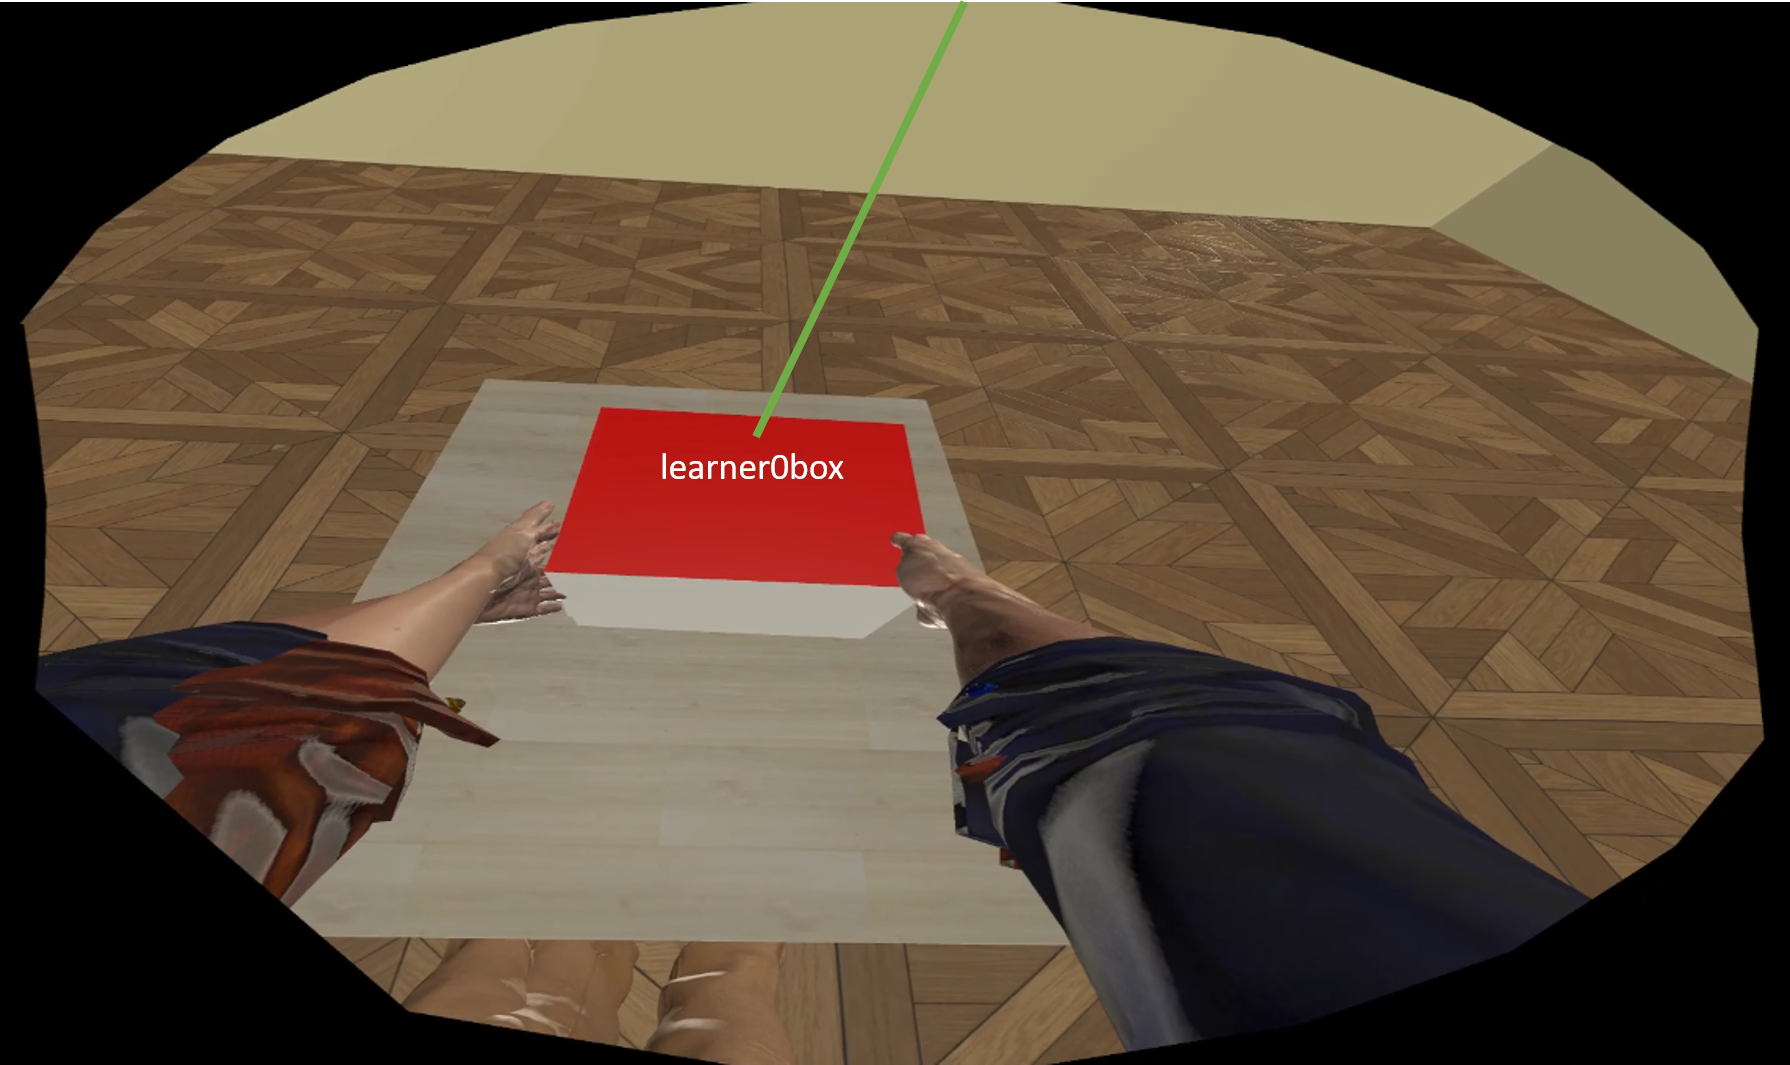
\includegraphics[width=\textwidth]{figures/focus.png}
	\caption[Focus assessment]{Visual focus assessment. Ego perspective of the learner. The ray is depicted with a green line.}
	\label{fig:focusAssessment}
\end{figure}
The virtual room the learner sees in \exgo\ is filled with tables, boxes, GVs and virtual copies of the learner. To assess on what the learner is focussing during the tasks, every object was given a name. In every frame, raytracing is performed. The ray's origin is the HDM and expands straight forward. The name of the object first hit by the ray is written into the log file. The name is coded with the position 0-4 (see positions in figure~\ref{fig:learner_positions}) and an object identifier (box, table, scale, GV, learner), compare figure~\ref{fig:focusAssessment}. A test revealed a systematic error of the ray pointing too high. To correct the discrepancy, the colliders of the objects were increased. The tables' and scales' collider height is increased by 20cm. The box' collider height was doubled. The learners' and GVs' avatar were wrapped into a capsule collider with a height 200cm of and a radius of 30cm. The values were determined by experimentation. To test the values, all subtasks were performed, and the object which was hit by the ray was displayed. The displayed name complied with the object in focus at nearly any point in time. Using an eye-tracker would increase the accuracy but was unavailable.


\subsection{(iv) Time Measurements}
The animation speed of the GV is determined by the distance between the learner and the GV (\textit{speed mechanic}). A slower played GV animation results in a longer task completion time. For ease of understanding, please consider the following two definitions: the time the task lasts without the \textit{speed mechanic} is defined as \textit{task norm duration} (TND). The time the learner needs more than the TND to fulfil the task is defined as \textit{over task norm duration} (OTND.)\\
OTND can draw conclusions about the learner's position in relation to the GV.
The tasks differ in the amount of time to be performed:
\begin{itemize}
	\item TND task 1: 172128ms
	\item TND task 2: 189040ms
	\item TND task 3: 176668ms
\end{itemize}
The OTND can be applied to specific subtasks, too. This measurement will mainly be used in the evaluation for triangulation.

Using the TCT for the evaluation of movements was previously done, for example by~\cite{onebody,YouMove,perspectivematters}.

\section{Qualitative Data Aquisition}
\label{sec:quali_logging}
The qualitative data assessment relies on one \textit{questionnaire} after each \textit{run} and a semi-structured \textit{interview} after all three \textit{runs}. The qualitative data assessment aims to determine the participant's impressions and opinions about the VPs. In the questionnaires, a different wording is applied to ease understanding. For example, the GV is called virtual teacher. 

\subsection{Questionnaire}
The \textit{questionnaire} (Appendix~\ref{appendix:questionaire}) starts with a question about the subjective overall performance of the learner. 
\begin{itemize}
	\item[Q1:] How accurate did your movements match with the virtual teacher?
	\item[A:] Likert scale from one (very good) to 7 (very poor)
	\item Linked research questions: RQ1.1.1-3, RQ1.4
	\item Data triangulation for (1-4,6)
\end{itemize}
The answer to this question gives insights into how accurate the participant judges the performed movements. Furthermore, this question can be used to determine if the qualitative accuracy complies with the participants' subjective opinion.\\
The next question aims to assess the user's subjective performance for the subtasks. The participant is asked to fill in a table. Each line represents a subtask. Each subtask can be rated on a Likert scale from 1 (very good) to 7 (very poor).
\begin{itemize}
	\item[Q2:] During the task, there were several smaller reoccurring movements, like pulling or lifting the box. Please rate these smaller movements to what extent you could follow the movements: 1 (very good) to 7 (very poor).
	\item[A:] Likert scale from 1 (very good) to 7 (very poor) for each subtask.
	\item Linked research questions: RQ1.1.1-3, RQ1.4
	\item Triangulation for (1-4,5,6)
\end{itemize}

\begin{figure}[H]
	\centering
	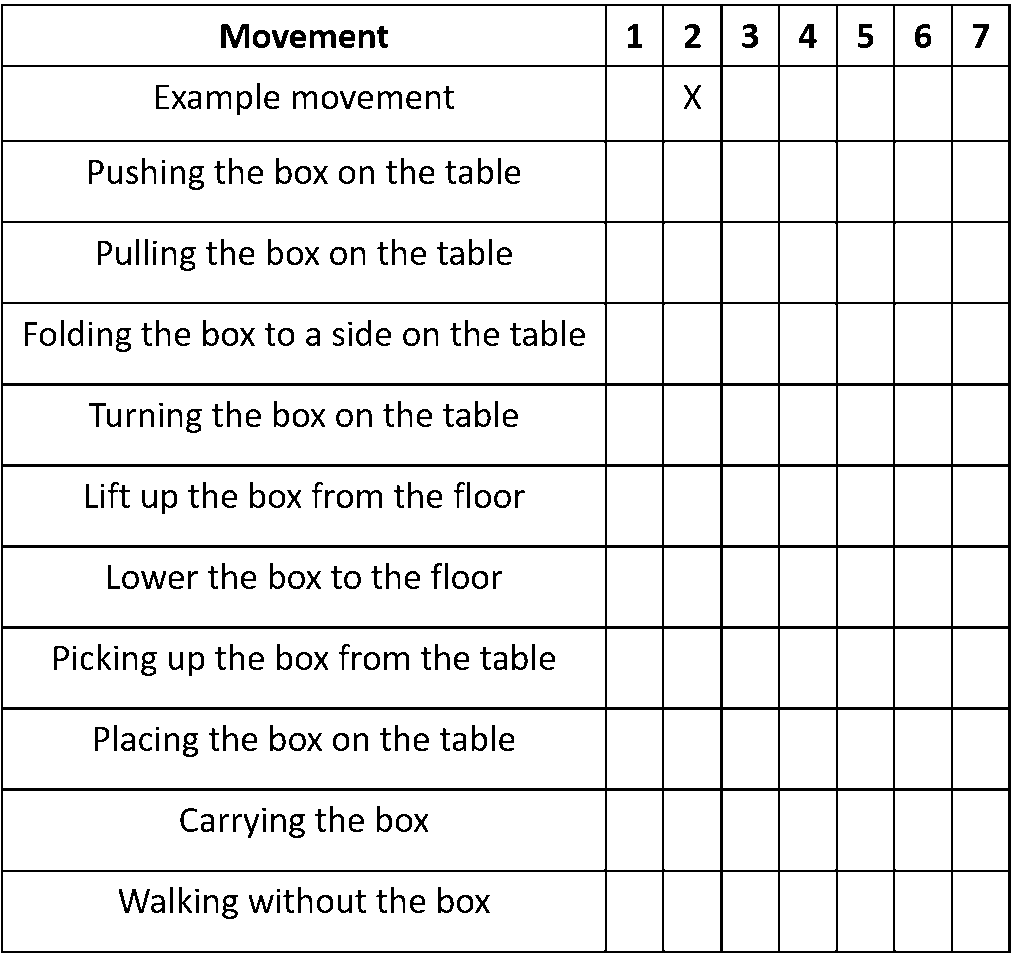
\includegraphics[width=0.6\textwidth]{figures/sub-task-rating.png}
	\caption[Rating template: subtasks]{Rating template for the subtasks.}
	\label{fig:subtaskrating}
\end{figure}

Beside the subjective opition about the participants' performance, the answers of Q2 can be used to be compared with the qualitative data.\\
Q3 aims to assess the subjective accuracy of the participants body parts.
\begin{itemize}
	\item[Q3:] Please rate to what extend you think you could align your body parts with the teachers body parts: 1 (very good) to 7 (very poor). 
	\item[A:] Likert scale from 1 (very good) to 7 (very poor) for each body part.
	\item Linked resarch questions: RQ1.1.1-3, RQ1.4
	\item Triangulation for (1-4,5,6)
\end{itemize} 
\begin{figure}[H]
	\centering
	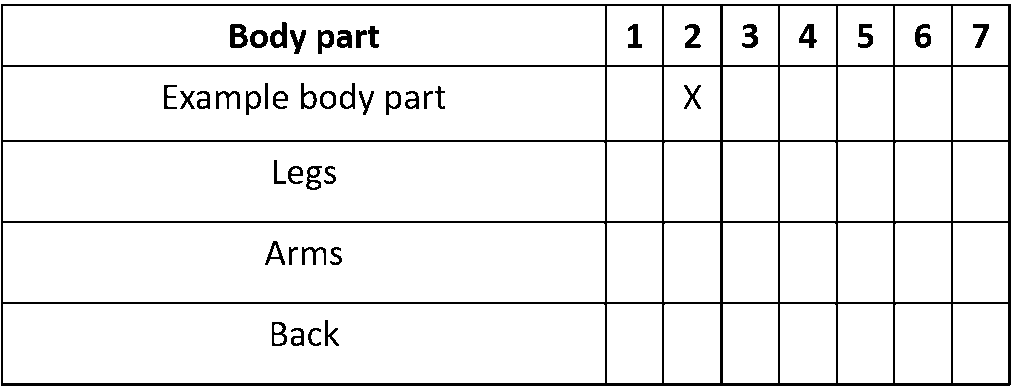
\includegraphics[width=0.6\textwidth]{figures/body-parts-acc.png}
	\caption[Rating template: body parts]{Rating template for the body parts.}
	\label{fig:bodypartsacc}
\end{figure}
Q3 assesses how good or bad the participant could perceive the body parts of the GV.\\
The last question is not handed to the participant. It serves as the basis for a subsequent semi-structured interview question. It gives the possibility to dig into extreme values of the questions answered before and into incidents that occurred during the performance of the task.
\begin{itemize}
	\item[Q4:] (As interview question) Did you have problems to follow the instructions? 
	\begin{itemize}
		\item E.g. because you could not see some body parts?
		\item E.g. bad perception related to the perspective?
		\item Go into extreme values of this questionnaire! 
		\item Address critical incidences!
	\end{itemize}
	\item[A:] Notes of participants statements.
\end{itemize}

\subsection{Semi-Structured Interview}
After all three \textit{runs}, the participant is interviewed with the help of the semi-structured interview guideline (Appendix~\ref{appendix:interview}). The guideline contains seven main questions, some with additional hints to dig deeper or to lower the participant's entry threshold to start reporting.
\begin{itemize}
	\item[Q5:] You saw three visual perspectives: ego-centric, exo-centric and the combination. What do you think about these perspectives?
	\begin{itemize}
		\item entry question, encourage participant to talk frank, address interesting statements.
	\end{itemize}
	\item[] Linked research question: RQ1.4
	
	\item[Q6:] Prioritise the perspectives by how accurate you could follow the movements. (1 best to 3 worst) 	
	\begin{itemize}
		\item Why did you prioritize this way?
	\end{itemize}
	\item[] Linked research question: RQ1.4
	
	\item[Q7:] Imagine you want to learn a movement in VR. Which perspective would you use for that?
	\begin{itemize}
		\item Or would you use a totally different one?
	\end{itemize}
	\item[] Linked research question: RQ1.4
	
	\item[Q8:] Which of the three perspectives was the easiest to understand? 
	\begin{itemize}
		\item Was there a perspective that confused you?
		\begin{itemize}
			\item What do you think caused the confusion?
		\end{itemize}
		\item Was there a perspective you did not understand right away?
	\end{itemize}
	\item[] Linked research question: RQ1.4
	
	\item[Q9:] What do you think are the advantages and disadvantages of the perspectives?
	\item[] Linked research question: RQ1.4
	
	\item[Q10:] Could you see some body parts better or worse in the perspectives?
	\begin{itemize}
		\item What about your legs, arms, back?
		\item Could you detect that during \textit{lift} and \textit{lower} you should squat?
		\item Could you detect that you should step back during \textit{push} and \textit{pull}?
	\end{itemize}
	\item[] Linked research question: RQ1.4
	
	\item[Q11:] Did you miss a feature?
	\begin{itemize}
		\item Dig for improvements for \exgo\ or experiment design.
	\end{itemize}
	
	\item[Q12:] (Space to ask for critical incidences if any occurred.)
\end{itemize}

\section{Experiment Procedure}
\label{sec:procedure}
\exgo\ is now complete, and the elements of the experiment design can be assembled with the technological elements of \exgo\ to form the final experiment procedure.\\
As soon as the participant enters the room, the participant receives a warm welcome to feel comfortable. The process starts with a welcome letter\footnote{Welcome letter, informed consent and demographic questionnaire partly informed by Daniel Schweitzer.} (appendix C), followed by the informed consent and a demographic questionnaire. In the meantime, \exgo\ is set up by choosing the condition, set the gender of the participant as well as the log is configured with the participant ID and task ID. After the demographic questionnaire, a spoken explanation about what is about to happen is given. Then the trackers are attached to the participant. The calibration process is explained. An explanation of the perspective is provided. Then, the first \textit{run} is started. \exgo\ gets started, the cameras and screen recording are set up, and the participant puts on the HMD. The participant is invited to calibrate. For calibration, the key C is pressed at the PC. To identify the camera recordings, a sign is held into the cameras. The task is started with the key S. During the \textit{run}, the study conductor pays attention to the cable of the HMD to keep the participant from stumbling over it. Furthermore, the participant is observed. After the \textit{run} ended, the HMD is removed. The participant fills in the \textit{questionnaire}. \textit{Run} two and three are conducted likewise. After all three \textit{runs}, the trackers are removed. The participant is interviewed. The payment is given, and the receipt signed. At the very end, the participant is thanked and said goodby. If it appears, doorstep talk is appreciated.

\section{Limitations}
\label{sec:limitations}
\exgo\ and the experiment is designed for a task that includes the handling of physical load. If the results of the experiment can be applied to movements without a physical load is questionable. Additionally, it cannot be assumed that the results of the experiment can be transferred for other physical loads that are significantly different in shape and weight. Furthermore, the exo-centric GV sometimes walk through artefacts (table, scale) of other GVs, which can confuse the experiment participant. The movements are not recorded by a professional, errors in ergonomic movements are possible. Furthermore, the subtasks have a specific magnitude. They can not stand for the same subtask with different magnitude. This means, for example, for \textit{lift}, the application of the outcome of the experiment for lifting up a box above the head is limited. Lastly, only a small number of participants participated in the formative tests to evaluate partial aspects of \exgo. Especially, the hip-box distance is not tested because multiple persons with different physique would be necessary. The artefact contribution of this master's thesis, locomotion guidance in the ego-centric VP, is limited by being evaluated by one participant.\\



